\textbf{Disminuir 8\% los precios de los productos de la categoría Furniture cuyo precio sea de \$600 a \$900. Aumentar en
un 5\% los precios de los productos de la categoría Technology y subcategoría Machines.} \vspace{.3cm}

Para esta consulta  use el video '07 Álgebra Relacional | Actualización | Operaciones de mantenimiento de datos', al final use esta consulta:

\begin{center}
    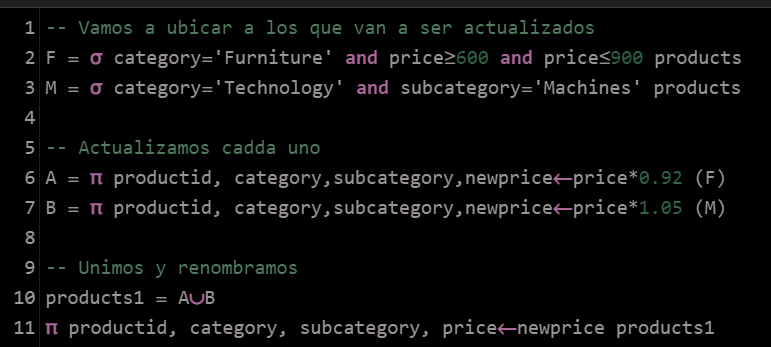
\includegraphics[width=14cm]{resources/pregunta2/3.5.1.png}
\end{center}

De manera que me quedo la siguiente Actualización:

\begin{center}
    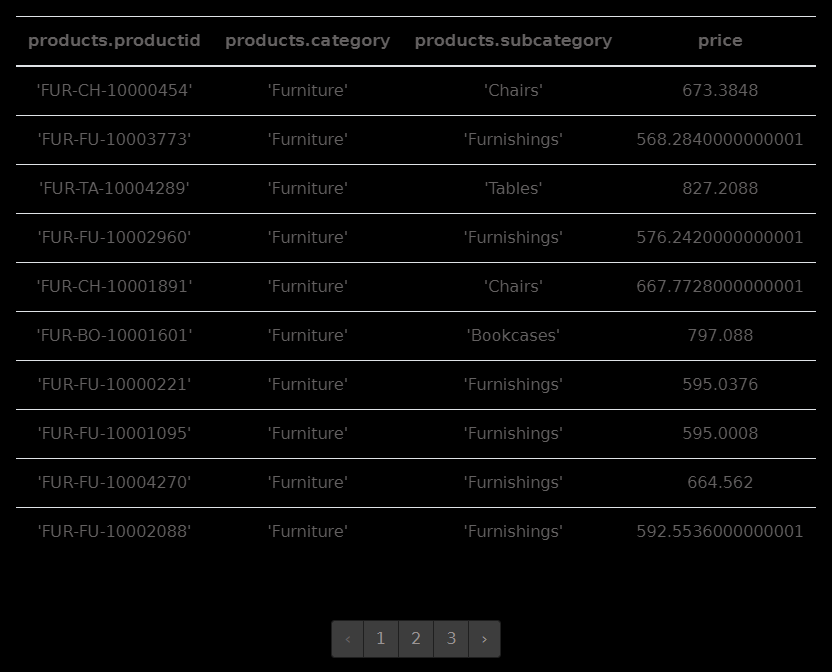
\includegraphics[width=14cm]{resources/pregunta2/3.5.2.png}
\end{center}

Ojo que esta solo contiene la tabla de los productos con los precios actualizados como se ve en el video, no contiene toda la lista de productos pero seria tan facil como eliminar las tuplas que se estan seleccionando, e insertar estas nuevas, no lo hice pues no lo hizo el profe :v.
\newpage        